  \section{Preliminaries}
\label{sec:preliminaries}
  This section defines the notation, the class of systems, and problem considered throughout the paper.

  \subsection{Notations}
  In the remainder of this text the following notation is adopted: 
Sets are italicized and capitalized (ex. $K$). 
The disjoint union of sets is defined as: $\coprod_{i\in I}K_i=\cup_{i\in I}K_i\times \{i\}$. 
Finite truncations of the set of natural numbers are expressed as \mbox{$\N_n:=\{1,\ldots,n\}$}. 
The set of continuous functions and absolutely-continuous functions supported on a compact set $K$ are represented as $\mathcal C(K)$ and $\mathcal C_{ab}(K)$, respectively. 
The ring of polynomials in $x$ is denoted by $\R[x]$, and the degree of a polynomial is equal to degree its largest multinomial; the degree of the multinomial $x^\alpha,\,\alpha\in \R_{\ge 0}^n$ is $|\alpha|=\|\alpha\|_1$; and $\R_d[x]$ is the set of polynomials in $x$ with maximum degree $d$. 
The dual to $\mathcal C(K)$ is the set of Radon measures on $K$, denoted as $\mathcal M(K)$, and the pairing of $\mu\in \mathcal M(K)$ and $v\in \mathcal C(K)$ is:
  \begin{align}
  \ip{\mu,v}=\int_{K}v(x)\,d\mu(x).
  \end{align}
The space of Radon probability measures on $K$ is denoted by ${\cal P}(K)$.
The Lebesgue measure is denoted by $\lambda$. 
Finally, supports of measures, $\mu$, are identified as $supp(\mu)$.

\subsection{System class description}
  The class of uncertain systems considered in this study consists of hybrid systems that conform to the following definition and undergo executions as described by Alg.~\ref{alg:execution}.
\begin{defn}[Inspired by \cite{Burden2015}]\label{def:system}
  A `quasi-uncertain' hybrid system is a tuple \mbox{$\mathcal H=(\mathcal J,\mathcal E,\mathcal D,\mathcal F,\mathcal G,\mathcal R,\Gamma)$}, where
  \begin{itemize}
    \item $\mathcal J$ is a finite set of indices of discrete states in of $\mathcal H$;
    \item $\mathcal E\subset \mathcal J\times \mathcal J$ is a set of two-tuples describing directed edges;
    \item $\mathcal D:=\coprod_{j\in\mathcal J} \mathrm{M}_j$ is a disjoint union of domains;
    \item $\Gamma:=\coprod_{j\in \mathcal J} \mu_{\theta_j}$ where $\mu_{\theta_j}\in \mathcal P(\Theta_j)$ describes the uncertainty associated with discrete state $j \in {\cal J}$;
    \item $\mathcal F:=\{\tilde f_j\}_{j\in \mathcal J}$ where \mbox{$\tilde f_j\in (\mathcal C(\mathrm{M}_j\times \Theta_j;\R))^{n_{x_j}}$} is a tangent vector to $\mathrm{M}_j$ at $(x,\theta)$,
    \item $\mathcal G:=\coprod_{p\in \mathcal E}\mathcal G_p$ is the disjoint union of guards; \mbox{$\mathcal G_{(i,j)}:=\{(x,\theta)\in \mathrm{M}_j\times \Theta_j\mid \text{algebraic constraints}\}$},
    \item $\mathcal R$ is the set of reset maps associated with each edge in $\mathcal E$; $R_{(i,j)}\colon \mathcal T\times \pi_{x}\mathcal G_{(i,j)}\rightarrow \mathcal T\times\mathrm{M}_j$ is a continuously differentiable injection; $\,R_{(i,j)}\in \mathcal C(\mathcal T\times \mathrm{M}_j)$ and denotes the transformation accompanying state transition.
  \end{itemize}
\end{defn}
A further qualification of the systems under consideration is warranted. It is assumed that upon reaching a guard, there is no ambiguity in into which discrete state the system transitions; this can be achieved by enforcing the next assumption.
\begin{assump}
    In each discrete state, the guards are mutually exclusive; i.e.
    \begin{align}
    \mathcal G_{(i,j)}\cap \mathcal G_{(i,k)}=\emptyset,\phantom{8}\forall (i,j),(i,k)\in \mathcal E, \forall j\ne k
    \end{align}
\end{assump}
In line with standard definition in literature related to switched systems, the discrete states are alternatively referred to as {\em modes} of the system. In addition, the systems considered are not allowed to undergo infinite mode transitions in a finite time-interval.
\begin{assump}
  $\mathcal H$ has no zeno execution.
  \label{assump:zeno}
\end{assump}
To complete the characterization of systems in $\mathfrak{U}$, a description of how the components in Defn.~\ref{def:system} are related is warranted. Algorithm~\ref{alg:execution} describes the finite-time execution ($t\in [0,T]$) of a hybrid system $\mathcal H$ as defined by Defn.~\ref{def:system} and whose states are denoted by $x$. The sequence of steps undertaken as the states evolve in accordance with Alg.~\ref{alg:execution} is briefly elaborated below.
\par
Suppose, without loss of generality (wlog.), that the system enters mode $j$ at time $t$. As a reminder, the dynamics of this system, $\tilde f_j$, is a function of a random parameter drawn from the distribution $\mu_{\theta_j}$; let this random variable take the value $\theta$. Consider a (non-hybrid) system, $\Sigma$, with states denoted by $\gamma$ whose dynamics is identical to that of $x$ in mode $j$, $\tilde f_j$; and let $\gamma$ have identical initial conditions as $x$ in mode $j$. The trajectory of the states of $\Sigma$ is given by an absolutely continuous function that is the solution to the ODE in Steps~\circled{5}\&\circled{6}. If $\gamma(s),\,s\in [t,T]$, does not satisfies any of the constraints that define the guards of mode $j$ of $\mathcal H$, then the trajectory of $x$ remains in mode $j$ and is identical to that of $\gamma$, and the execution is terminated; otherwise, $\mathcal H$ undergoes a mode transition. Steps~\circled{7}--\circled{11} isolates the first hitting-time of a guard of mode $j$ and resets $\mathcal H$ to a new mode whereafter the same procedure is repeated until $t=T$.
\par
\begin{algorithm}[!t]
\small
 {\bf Initialization:} $t=0,\,j\in \mathcal J,\,(x_0,j)\in \mathcal D,\,x(0)=x_0$\;
 \While{1}{
 {\em Let} $\theta$ be drawn according to $\mu_{\theta_j}$\;
 {\em Let} $\gamma\colon [t,T]\rightarrow \mathrm{M}_j$, abs. ct. st.\\\hspace{.2in}
 $\dot \gamma(s)=\tilde f(\gamma(s),\theta)$ $\lambda_t^{\text{\tiny a}}$-a.e., $s\in [t,T]$\\\hspace{.2in}
 $\gamma(t)=x(t)$\;
 $\Lambda_{(j,t)}:=\{r\in [t,T]| \exists (j,k)\in \mathcal E \text{ st. } (\gamma(r),\theta)\in \mathcal G_{(j,k)}\}$\;
 \eIf {$\Lambda_{(j,t)}\ne \emptyset$}{%\\\hspace{.2in}
    $t':=\min \Lambda_{(j,t)}$, $k$ st. $\gamma(t')\in \pi_{x}\mathcal G_{(j,k)}$\\\hspace{.2in}
     $x(s)\leftarrow \gamma(s)$, $\forall s\in [t,t')$\\ \hspace{.2in}
    $t\leftarrow t',\,x(t')\leftarrow R_{(j,k)}(\gamma(t')),\,j\leftarrow k$
 }
 {
 $x(s)=\gamma(s),\,\forall s\in [t,T]$\;
 Stop\;
 }
 }
 \caption{Execution of $\mathcal H$}
 \label{alg:execution}
 $^a$where $\lambda_t$ is the Lebesgue measure on $[t,T]$
\end{algorithm}
Of key note in the system execution is the fact that the uncertainty does not evolve with time; changes to the value that the uncertainty takes is triggered with system mode resets. In spite of this peculiar requirement, $\mathfrak{U}$ is quite rich and includes many physical systems; to better elucidate the properties of systems in this class, two representative examples---a simple 1D pedagogical example, and a 2D representative of walking models---are presented hereafter.
\begin{example}[1-D linear dynamics]
\label{example:1D}
One of the simplest linear examples in $\mathfrak{U}$ has dynamics described by
\begin{align}
	\dot x = -0.7x+0.2\theta-0.1,
\end{align}
where \mbox{$x(t)\in [-1,1]$} and $\theta\in [-1,1]$ is an uncertain, unknown parameter; the uncertain parameter can be thought of as having arisen due to structural modeling errors or as a result of reducing a singular-perturbed system. Note that this system is not a hybrid system; however, it can be hybridized. One way to achieve this is by setting $n_m=1$ and using placing a guard $\mathcal G_{(1,1)}$ at $x(t)=-1$ with a corresponding reset map $x\mapsto -x$.
\end{example}
\begin{figure}[!t]
\centering
  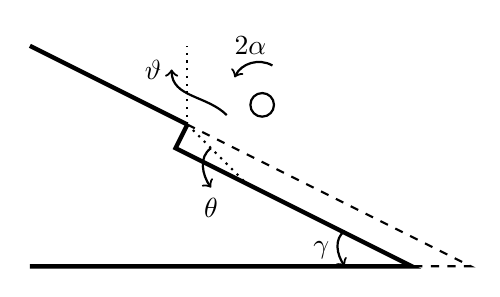
\begin{tikzpicture}
    \draw[-,ultra thick] (0,2) to (2,1);
    \draw[dashed, thick] (2,1) -- (5.6,-0.8)-- (4.85,-.8);
    \draw[ultra thick] (2,1) to (1.85,0.7) -- (4.85,-0.8)--(0,-0.8);
    \draw[thick] (2.95,1.25) circle (.15cm);
    \spoke{(2.95,1.25)}{-75};
    \spoke{(2.95,1.25)}{-15};
    \spoke{(2.95,1.25)}{45};
    \spoke{(2.95,1.25)}{105};
    \spoke{(2.95,1.25)}{165};
    \spoke{(2.95,1.25)}{-135};
    \draw[dotted,thick] (2,1) -- (2,2);
    \draw[dotted, thick] (2,1) -- (2.75,.25);
    \draw[->,thick] (2.3, 0.7) to [out=-145, in =125] (2.3,0.2) node[below] {$\theta$};
    \draw[->,thick] (4,-.35) to  [out=-145, in =125] (4,-0.8);
    \node at (3.7,-0.6) {$\gamma$};
    \draw[->, thick] (3.08,1.75) to [out=150, in =65] (2.6,1.6);
    \node at (2.8,2) {$2\alpha$};
    \draw[->,thick] (2.5,1.12) to [out=135, in =-90] (1.8,1.7) node[left]{$\vartheta$};
  \end{tikzpicture}
  \caption{Schematic of the rimless wheel with $\theta$ being the disturbance.}
  \label{fig:rw_schematic}
\end{figure}
\begin{example}[Planar rimless wheel (PRW)]
\label{example:rw}
  The planar rimless wheel---constituted by a massless axle to which $n$ (angularly) equidistant spokes are connected---is one of the simplest models of legged locomotion. Figure~\ref{fig:rw_schematic} presents a schematic of a rimless wheel---with spokes separated by an angle $2\alpha$---rolling down an infinite wedge. The PRW is, by definition, a hybrid system consisting of one mode; every-time the spoke make contact with the surface of wedge, the system undergoes a rest as the pivoting leg, and the origin of the local generalized coordinates changes. Between resets, the dynamics of the PRW is described by
\begin{align}
  \begin{bmatrix}
    \dot \vartheta& \ddot\vartheta
  \end{bmatrix}'=\begin{bmatrix}
    \dot\vartheta&\sin(\vartheta)
  \end{bmatrix}',
\end{align}
where $\vartheta$ is the angle between the pivoted spoke and the vertical located at the stationary leg. Once the marching spoke makes contact with the terrain, the states are reset using the reset map
\begin{align}
R_{(1,1)}(t,\vartheta^-,\dot \vartheta^-)=\begin{bmatrix}t&
    2\gamma-\vartheta^-&
    \cos(2\alpha)\,\dot\vartheta^-
  \end{bmatrix}'.
\end{align}
For a PRW rolling down a flat (constant slope) wedge, at the instance when the marching spoke makes contact with the wedge, and the system undergoes a reset, the states of the system satisfy the following condition
\begin{align}
\vartheta = \gamma+\alpha.
\end{align}
For a PRW rolling down a wedge with an uneven ramp with the relative slope between the pivoted leg and the contact point of the marching leg, $\theta$, the guard, $\mathcal G_{(1,1)}$ is defined as follows
\begin{align}
\mathcal G_{(1,1)}=\{x\mid x=\gamma+\alpha+\theta\}.
\end{align}
Observe that as the PRW continues to roll, the undulations in the surface can change and hence the random variable, $\theta$, will likely take different values as the system resets.
\end{example}
\subsection{Problem description}
The objective of this work is to estimate the {\em largest set of initial conditions} from which all state trajectories of a hybrid quasi-uncertain system reach the terminal set $X_T$ in a pre-specified time, $T$.
\par
Depending on $\mathcal E$, there may be more than one trunk through which state trajectories can reach the terminal set. Consequently, the problem can be re-stated, with specificity, as wanting to find the largest set of initial conditions in each mode, $X_{(0,j)},\,\forall j\in \mathcal J$, that can reach $X_T$ where $X_{(0,j)}$ is given by
\begin{align}
\begin{aligned}
     X_{(0,j)}:=\{x_0\in \mathrm M_j\mid \forall x=\mathcal H(x_0,[0,T]) \\\,x(T)\in X_T\}
     \label{eq:brs}
\end{aligned}
\end{align}
Observe that, by definition, for systems from $\mathfrak{U}$, if $X_{(0,j)}$ is the largest non-empty BRS in mode $j$, then all initial conditions from $X_{(0,j)}$, must reach $X_T$ at time $T$, regardless of the number of mode transitions that may occur in the interim and for every possible concomitant sequence of parametric uncertainty.
\par
For convenience, hereafter the times at which the system's state is relevant is denoted by the set $\mathcal T:=[0,\,T]$, and the projections of $X_T$ onto every mode, $j$, is denoted by $X_{(T,j)}$.
